\chapter{Ala}
Començant pels càlculs més bàsics, s'estudia el comportament de l'ala com a cos aïllat. En els següents apartats es descriuen l'efecte de l'angle de twist en l'aerodinàmica de l'ala i la variació de la resistència aerodinàmica en funció de la sustentació.

\section{Angle de sustentació nul·la}
L'únic paràmetre geomètric de l'ala que queda per determinar és l'angle de twist. Per tal de fer-ho, és útil calcular l'angle de sustentació nul·la de la secció central de l'ala per a diferents valors d'aquest angle, concretament en el rang de -8 a 0$^{\circ}$. L'algoritme seguit per fer-ho es mostra a continuació.
\begin{figure}[H]
	\centering
	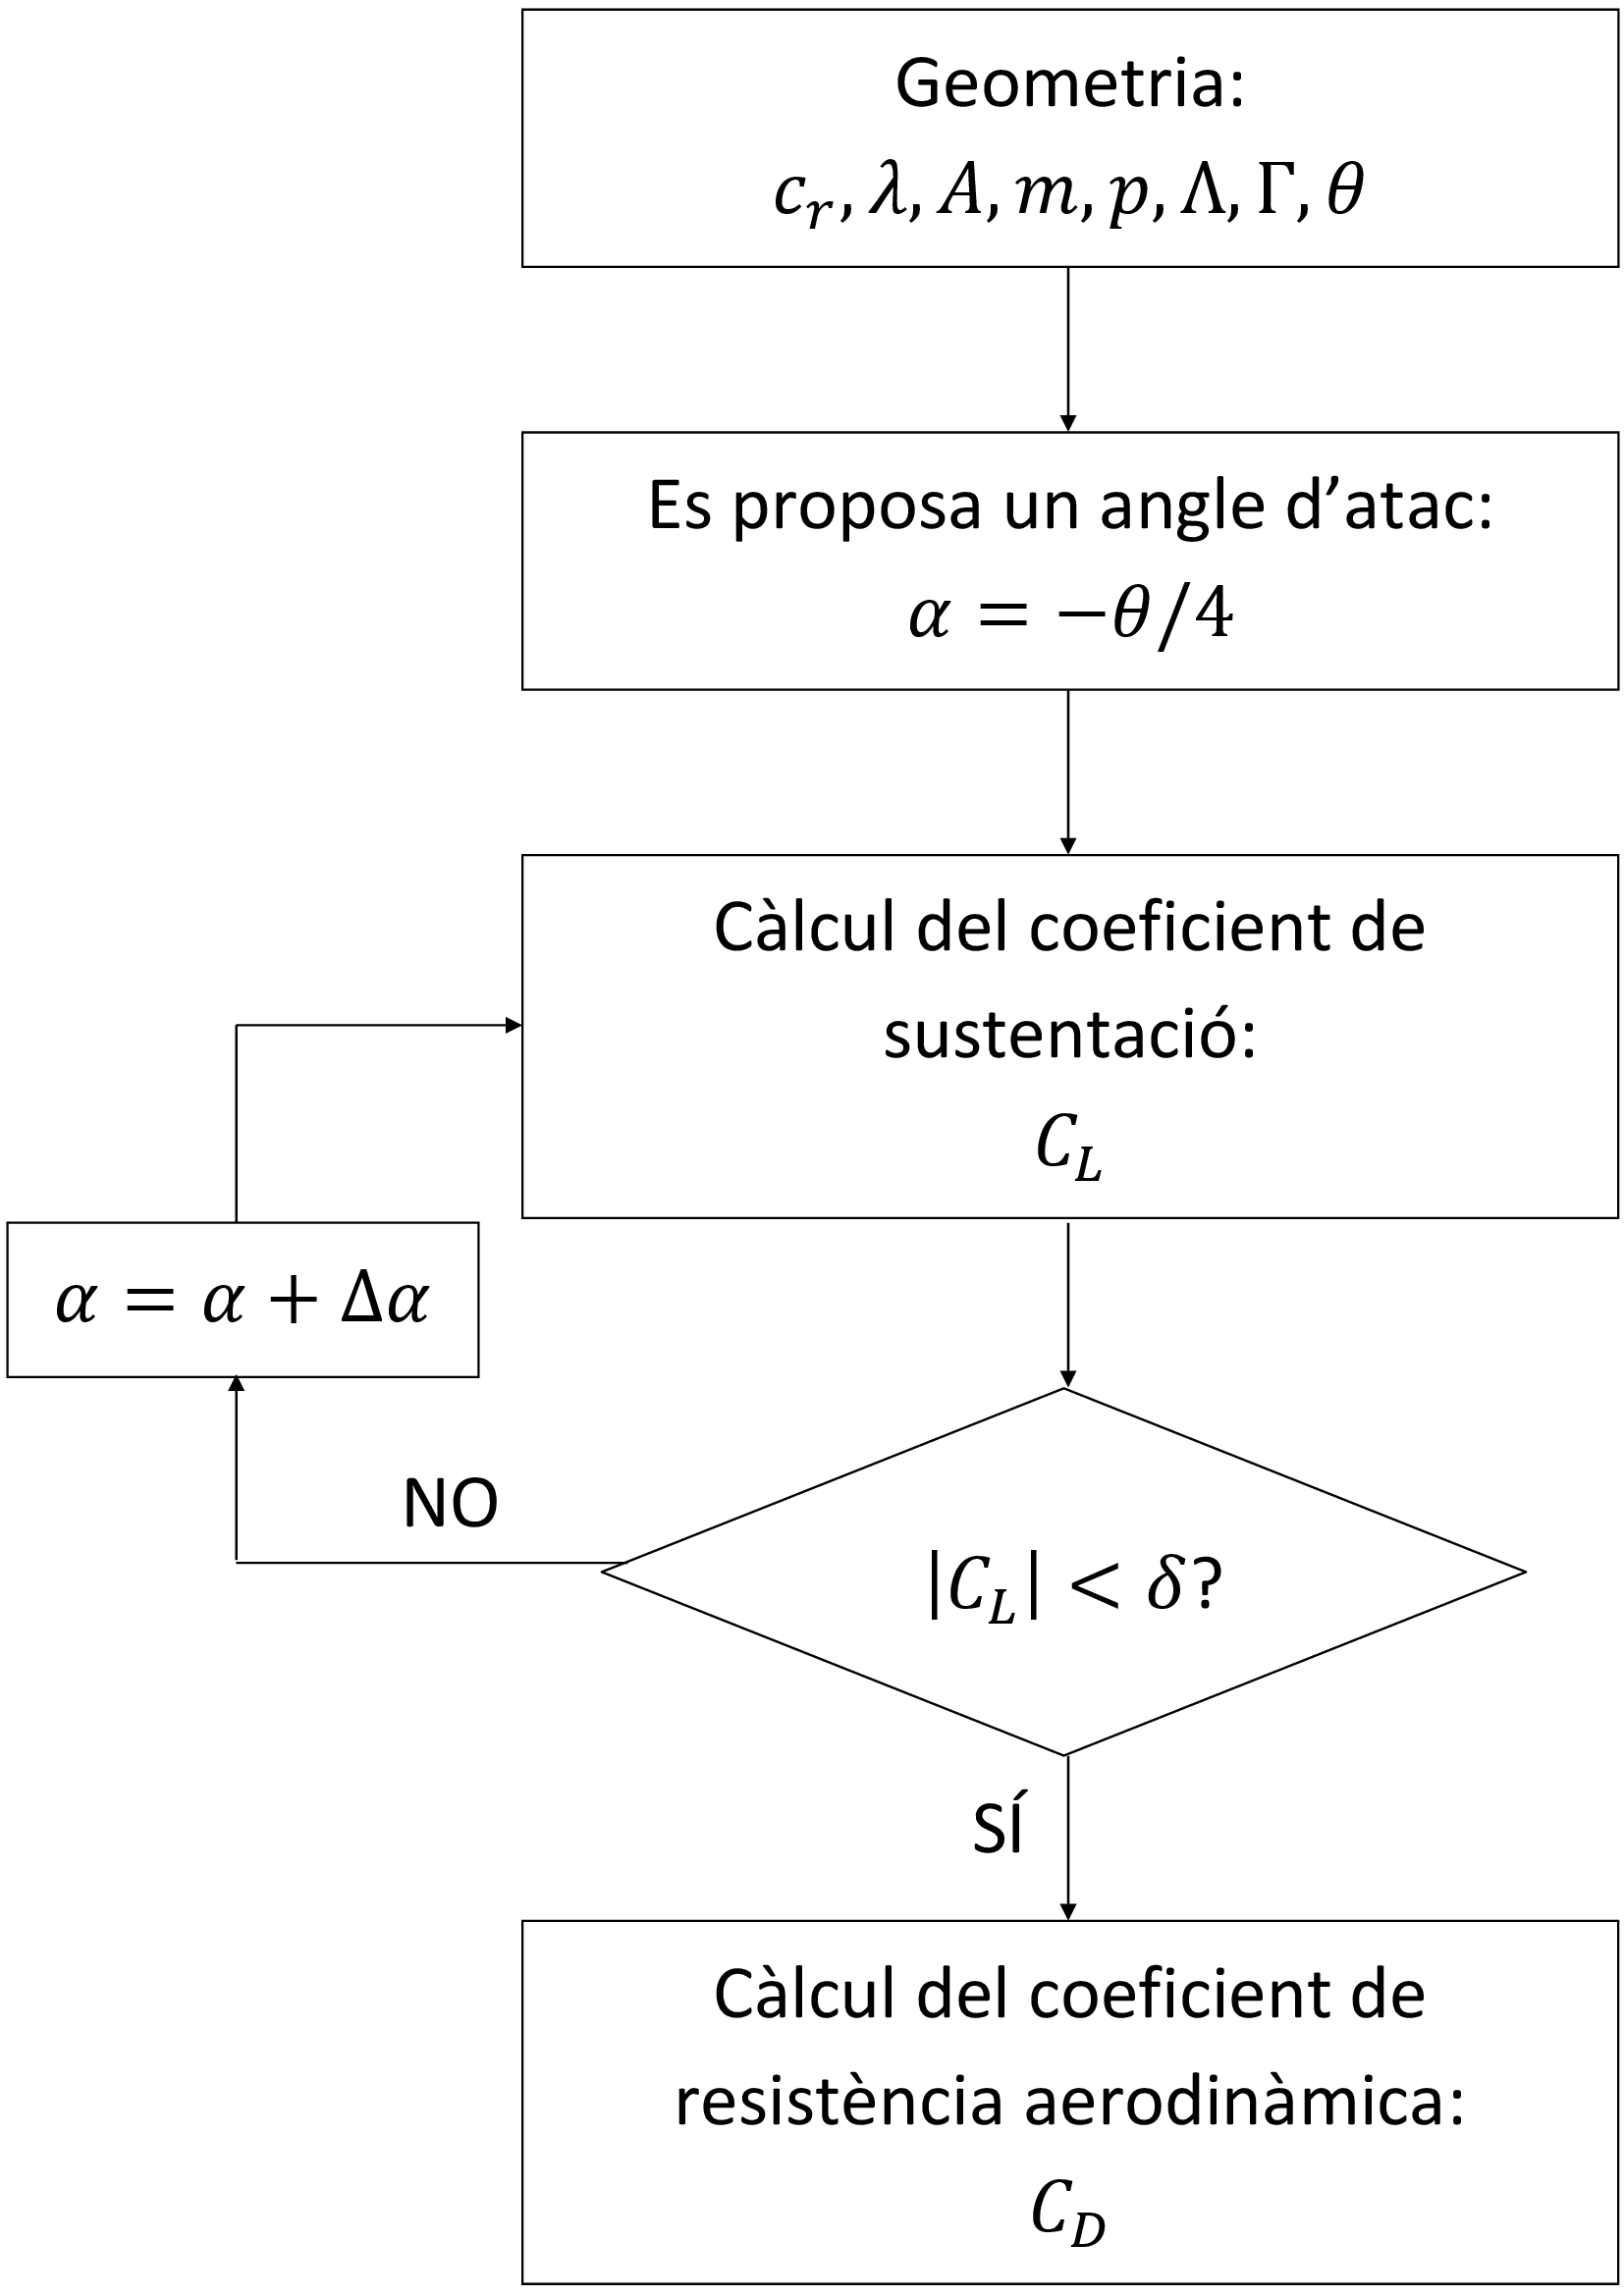
\includegraphics[scale=0.1]{./plots/algoritmeZLangle}
	\caption{Algoritme de càlcul de l'angle de sustentació nul·la}
\end{figure}

Com s'observa, es tracta d'un algoritme iteratiu. Un cop introduïdes les dades geomètriques del planejador, es proposa un angle d'atac inicial per tal que el programa pugui començar a fer càlculs. Es calcula el coeficient de sustentació i es comprova si aquest és més petit que una tolerància proposada, en aquest cas $\delta=10^{-3}$. Si no és així, es varia l'angle d'atac en un increment que depèn del valor del coeficient de sustentació calculat anteriorment. Aquest procés es va repetint fins que s'obté un coeficient de sustentació més petit que $\delta$.

Finalment, el següent pas és el càlcul del coeficient de resistència per a l'angle d'atac obtingut. En aquest càlcul s'imposa que la sustentació és nul·la, per evitar possibles errors deguts a la tolerància.

\begin{figure}[h]
	\centering
	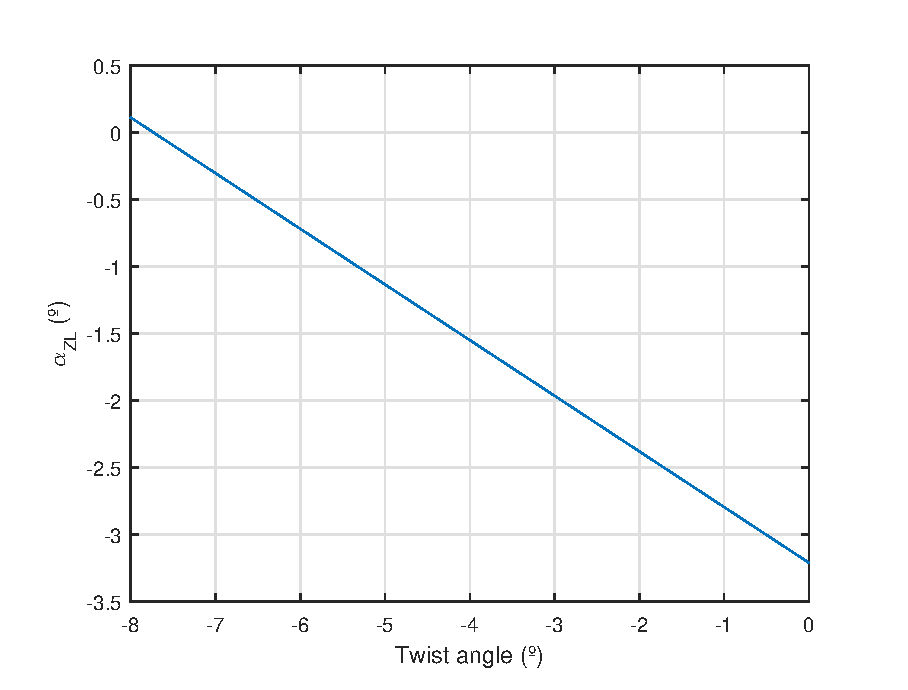
\includegraphics{./plots/zlangle}
	\caption{Angle de sustentació nul·la per diferents valors de twist}
	\label{zla}
\end{figure}

Els resultats d'aquest estudi es resumeixen en la figura \ref{zla}. Com es pot observar, la dependència entre l'angle de twist i l'angle de sustentació nul·la és completament lineal. A mesura que el twist es torna més negatiu, l'angle de sustentació nul·la augmenta. És a dir, a mesura que s'incrementa el twist, l'angle mínim necessari per tal de sustentar també es veu incrementat.

Tenint en compte aquests resultats, es determina que per a tal de tenir el màxim de sustentació possible, el millor angle de twist és el que permet un angle de sustentació nul·la més baix. Per tant, s'escull un twist de $\theta=0^{\circ}$.

\subsection{Resistència aerodinàmica}
A l'hora de calcular l'angle de sustentació nul·la per a diferents valors de twist, també s'ha determinat el coeficient de resistència aerodinàmica per tal d'estudiar la seva variació en funció d'aquest paràmetre.

Com és de suposar, ja que la sustentació és nul·la, la resistència induïda també és nul·la. No obstant, cal tenir en compte la resistència paràsita. Aquesta, com s'observa a la figura \ref{cdpar}, no depèn de l'angle de twist, ja que no depèn de la sustentació, i pren un valor constant de $C_{D}=C_{D_{0}}=0.0063$.

\begin{figure}[h]
	\centering
	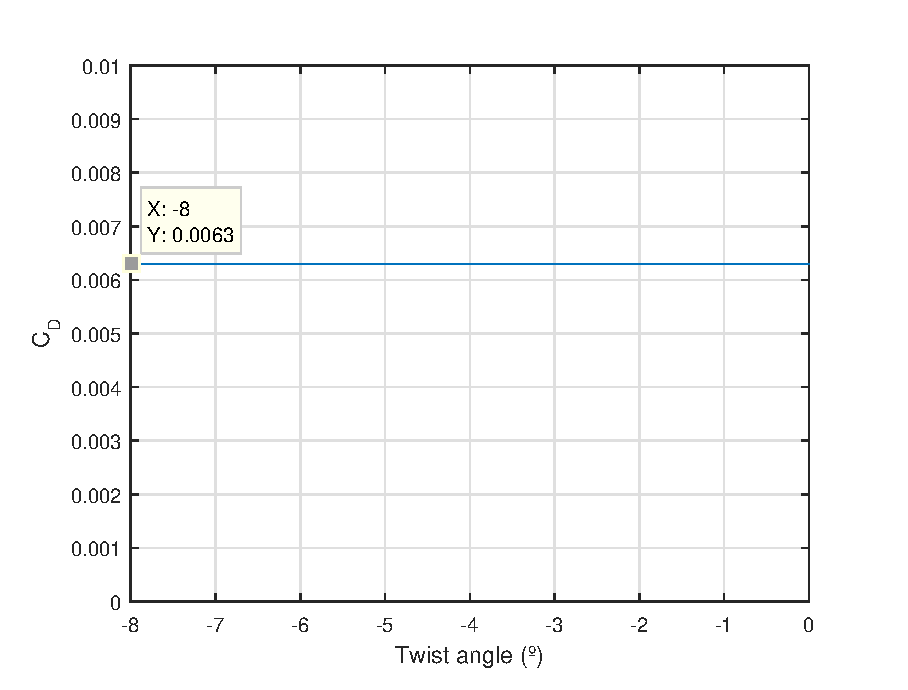
\includegraphics{./plots/cdparasita}
	\caption{Resistència aerodinàmica en angle de sustentació nul·la}
	\label{cdpar}
\end{figure}

Veient que la resistència paràsita no depèn del valor de twist, aquests resultats només serveixen per reafirmar la decisió presa en l'apartat anterior d'assignar al planejador un angle de twist de 0$^{\circ}$.

\section{Corba polar}
Finalment, per completar l'anàlisi de l'aerodinàmica de l'ala, és necessari calcular els coeficients de sustentació i de resistència aerodinàmica. Per tal d'obtindre diversos valors significatius, aquests s'estudien per a diversos angles d'atac, de 0 a 10$^{\circ}$. L'algoritme seguit és el que s'il·lustra a la secció \ref{algoritmeala}.

\begin{figure}[h]
	\centering
	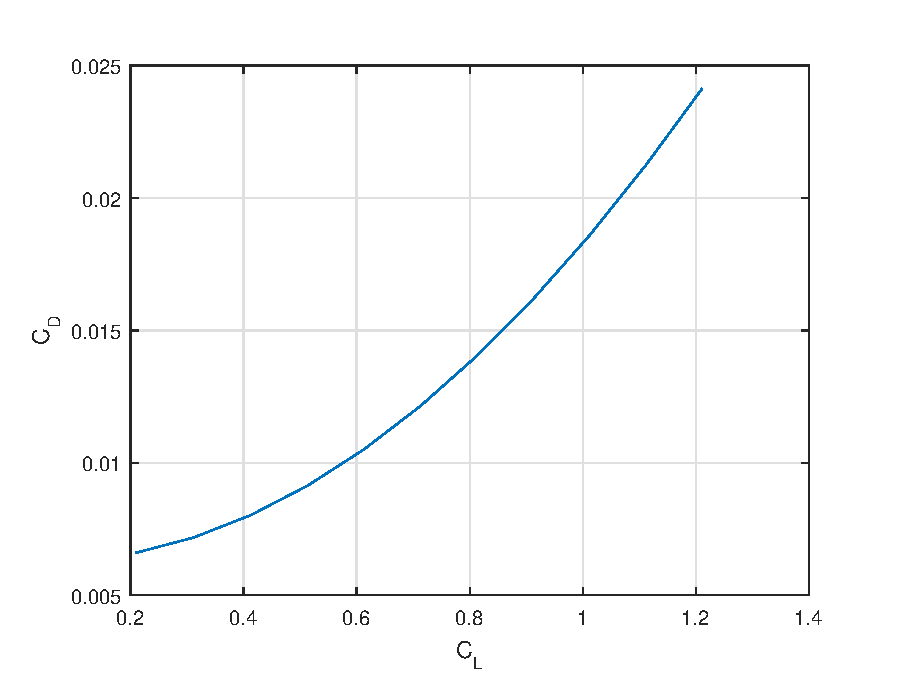
\includegraphics{./plots/polarcurve}
	\caption{Corba polar ($C_{D}$ vs. $C_{L}$)}
	\label{polar}
\end{figure}

Com s'observa a la figura \ref{polar}, la representació gràfica del coeficient de resistència aerodinàmica en funció del coeficient de sustentació pren forma de paràbola, tal i com s'esperava.